
\subsection{Operads}

Our goal in this paper was to present an initial formalization of quantum
computing in the language of TQFTs and geometric structures supported on them.
Hence our constructions are mostly based on combinatorial and geometric data
that can be associated with cobordisms. Nevertheless, one cannot but notice the
similarity of transport graphs and, more visibly, cobordisms themselves with
operads. As a start, consider the operad of rooted trees whose non-root vertices
are all leaves and where composition is given by gluing the root of a tree with
one of the leaves of another tree \cite{WhatOp}. Of course, for each leaf, we
get a different composite which is different from gluing the operation for
cobordisms, at first sight. An example is shown below, where the subscript of
the composition sign indicates the leaf chosen for the gluing.
\[\begin{tikzpicture}

\colvert{black}{-2, 0}{a}
\colvert{black}{-3, 0.5}{a1};
\colvert{black}{-3, 0}{a2};
\colvert{black}{-3, -0.5}{a3};
\draw (a1) -- (a);
\draw (a2) -- (a);
\draw (a3) -- (a);

\lblvert{-1.5, 0}{comp}{$\circ_2$}

\colvert{black}{0, 0}{a}
\colvert{black}{-1, 0.25}{a1};
\colvert{black}{-1, -0.25}{a2};
\draw (a1) -- (a);
\draw (a2) -- (a);

\lblvert{0.5, 0}{eq}{$=$}

\colvert{black}{3, 0}{a}
\colvert{black}{2, 0.5}{a1};
\colvert{black}{2, 0}{a2};
\colvert{black}{2, -0.5}{a3};
\draw (a1) -- (a);
\draw (a2) -- (a);
\draw (a3) -- (a);

\colvert{black}{1, 0.25}{a4};
\colvert{black}{1, -0.25}{a5};
\draw (a4) -- (a2);
\draw (a5) -- (a2);

\end{tikzpicture}
\]

However, we notice that the difference of this situation with transport graphs
or cobordisms is artificial for we could define composition operations for
transport graphs and cobordisms parametrized by their inputs and outputs similar
to the case of operads. Note, however, that we need to handle the gluing of
multiple outputs to inputs in various combinations. For this, we informally
introduce a modification of operads.

\begin{defn}[Multioperad]
Let $\s{C}$ be any (not necessarily symmetric) monoidal category and
$P = \set{P(n, m)}_{n, m \in \N}$ be a
collection of objects of $\s{C}$. For any $n \in \N$ and $1 \leq i \leq n$,
let $I = \set{i, i + 1, \dots, i + m} \subset \set{1, \dots, n}$. For each
such $n$ and $I$ as well as some $n' \in \N$, suppose there is a morphism in
$\s{C}$ as follows:
\[
  \circ_I : P(n, m) \tensor P(n', n) \to P(n', m)
\]
Then, with some coherence conditions we have not explored, we will call
$P$ a multioperad in $\s{C}$.
\end{defn}

\begin{exm}
Consider the same diagram above giving an example of operads of trees. This
diagram is an example of a (pre)transport graph if we direct the edges and
colour the vertices! Take $\s{C}$ to be the monoidal category of transport
graphs and transport homomorphisms and composition to be gluing of targets of
transport graphs to a contiguous subset of the source of another
transport graph.
We note that the only difference with the definition given
above with an operad is that the composition operation
here is parametrized by a ``segment'' of the gluing site as opposed to a single
input, as is the case with operads. We give another example below to clarify the
difference:
\[\begin{tikzpicture}

\colvert{green!55!black}{1, 2.5}{c}
\colvert{blue!55!black}{1, 1.75}{cc}
\colvert{blue!55!black}{0, 3.25}{c1}
\colvert{green!55!black}{0, 2.75}{c2}
\colvert{blue!55!black}{0, 2.25}{c3}
\colvert{blue!55!black}{0, 1.75}{c4}
\midarrow{c1}{c}
\midarrow{c2}{c}
\midarrow{c3}{c}
\midarrow{c4}{c}
\midarrow{c4}{cc}

\lblvert{2, 2.5}{comp}{$\circ_{\set{2, 3}}$}

\colvert{green!55!black}{4, 3}{a}
\colvert{blue!55!black}{3, 3.5}{a1}
\colvert{blue!55!black}{3, 3}{a2}
\colvert{blue!55!black}{3, 2.5}{a3}
\midarrow{a1}{a}
\midarrow{a2}{a}
\midarrow{a3}{a}

\colvert{blue!55!black}{4, 2}{b}
\colvert{green!55!black}{3, 2}{b1}
\colvert{blue!55!black}{3, 1.5}{b2}
\midarrow{b1}{b}
\midarrow{b2}{b}
\midarrow{a3}{b}

\lblvert{5, 2.5}{comp}{$=$}

\colvert{green!55!black}{8, 2.5}{c}
\colvert{blue!55!black}{8, 1.75}{cc}
\colvert{blue!55!black}{7, 3.25}{c1}
\colvert{green!55!black}{7, 2.75}{c2}
\colvert{blue!55!black}{7, 2.25}{c3}
\colvert{blue!55!black}{7, 1.75}{c4}
\midarrow{c1}{c}
\midarrow{c2}{c}
\midarrow{c3}{c}
\midarrow{c4}{c}
\midarrow{c4}{cc}

\colvert{blue!55!black}{6, 3.5}{a1}
\colvert{blue!55!black}{6, 3}{a2}
\colvert{blue!55!black}{6, 2.5}{a3}
\colvert{green!55!black}{6, 2}{b1}
\colvert{blue!55!black}{6, 1.5}{b2}
\midarrow{a1}{c2}
\midarrow{a2}{c2}
\midarrow{a3}{c2}
\midarrow{b1}{c3}
\midarrow{b2}{c3}
\midarrow{a3}{c3}

\end{tikzpicture}\]
Notice that the composition glues the output vertices of the right operand
with the second and third vertices of the left operand, as indicated by
$\circ_{\set{2, 3}}$.
In this example, we also considered coloured vertices and hence what we really
require is a coloured variant of multioperads, in the same spirit of introducing
colours to ordinary operads. Gluing different coloured
vertices requires some intermediary -- say, an arrow from green to blue -- but
the the choice of this intermediary is not unique. Hence, it is easier to
require gluing of vertices of the same colour only.
\end{exm}

\begin{exm}
Of course, thick tangles admit the same structure. Given the output boundary
components of one thick tangle, we can choose a matching collection of input
boundary components of another and glue accordingly.
\end{exm}

Note, in particular, the similarity with cyclic operads
\cite{ModOp}. Recall that a cyclic operad $P$ is roughly an operad with the
action of the symmetric group $S_n$ on $P(n)$ replaced by an action of
$S_{n + 1}$. This effectively conflates the ``inputs'' and ``outputs'' of an
operad ``element''. Here, however, we take a much more elementary approach --
simply allow multiple inputs and multiple outputs. The other difference is that
a multioperad should not require symmetry in a monoidal category for our
categories of thick tangles and transport graphs are not equipped with symmetry.

Next, we comment on a possible connection to modular operads \cite{ModOp}.
A modular operad is roughly a cyclic operad which allows for the gluing of
``inputs'' and ``outputs'' of the same object \cite{Giansiracusa}.
This formalism is not present in the our setting, but we can try to introduce
something similar, although in a non-unique way. Consider the simple example
below. Here, we wish to glue the first and only output to the first input, say.
\[\begin{tikzpicture}
\colvert{green!55!black}{1, 3}{a}
\colvert{green!55!black}{0, 3.5}{a1}
\colvert{blue!55!black}{0, 3}{a2}
\colvert{blue!55!black}{0, 2.5}{a3}
\midarrow{a1}{a}
\midarrow{a2}{a}
\midarrow{a3}{a}

\draw[->] (2, 3) to (3, 3);

\colvert{green!55!black}{5, 3}{a}
\colvert{blue!55!black}{4, 3}{a2}
\colvert{blue!55!black}{4, 2.5}{a3}
\midarrow{a2}{a}
\midarrow{a3}{a}

\draw[->] (a) edge[loop] node {} (a);

\end{tikzpicture}\]
If we were to do this directly, it would introduce a loop in the graph which
contradicts our condition on transport graphs. In more general situations, we
would introduce cycles. Introducing cycles in a graph upsets the level ordering
of our graphs and hence the algorithm for extracting linear maps by parallel
transport. To remedy this, we must modify our definition of transport
graph and our algorithm to be able to interpret and handle cycles in a
satisfactory way.
Furthermore, it is not only interesting, but also necessary to fit the addition
of cobordisms to the operadic formalism for a full translation of our framework
to operad theory.

We observe that the gluing constructions that have worked so far for transport
graphs, also work for bundles with connection as well so that our framework for
quantum computing could be treated in this operadic formalism. However, making
all the details precise and handling the issues discussed in the previous
paragraph is beyond the scope of the current work. Nevertheless,
these preliminary observations hint at various possibilities.
Modular operads as developed by Getzler and Kapranov generalize
Kontsevich's graph complexes \cite{ModOp}. Perhaps, we can find an
interpretation of these graph complexes or of the graphs defined in
\cite{ModOp} as parallel transport machinery, leading
to a solution of the self-gluing problem for transport graphs.
It if of interest to fully flesh out such connection to
modular operads for this could lead to the
application of Chern-Simons theory to the quantum computing framework
developed in this paper. On the other hand, an approach to cobordism
theory using coloured operads \cite{CobOp} has been used to categorify $sl_n$
quantum invariants. The operadic approach to transport graphs on manifolds
with connections might be one way to relate categorification in
representation theory with quantum computing.

